% 对照原 PPT 第1—30页重排；新增模板结束页。正文与公式可编辑。
\campusmaketitle
% 原第2页
\begin{frame}[t]{情境引入：怎样表示函数}
把一个函数的\alert{对应关系和定义域}交代清楚的办法，就是表示函数的方法。
\vspace{3mm}
\dinosay{你知道哪些表示函数的方法？}
\pause
\begin{block}{三种主要方法}
解析法：用数学表达式表示。\par
列表法：用函数表表示。\par
图象法：用函数图象表示。
\end{block}
数学研究的对象是抽象的，把它表示出来，才便于研究。
\end{frame}
% 原第3页
\begin{frame}[t]{新知探索：解析法}
\begin{block}{解析法}
用解析式来表示函数的方法。
\end{block}
把常量和表示自变量的字母用一系列运算符号连接起来得到的式子，叫作\alert{解析式}，也叫函数表达式或函数关系式。
\vspace{3mm}
例如，正方形面积 $S$ 是边长 $x$ 的函数：
\[S=x^2,\qquad x\in(0,+\infty).\]
\dinosay{写出对应关系时，别忘了定义域。}
\end{frame}
% 原第4页
\begin{frame}[t]{例题解析：水库大坝的横断面}
\begin{columns}[T,onlytextwidth]
\begin{column}{.73\textwidth}
某地在山区修建水库大坝，坝高随山势起伏在 $10\,\mathrm m$ 到 $50\,\mathrm m$ 之间变化。坝体横断面为梯形，上底 $a=30\,\mathrm m$，下底 $b$ 与坝高 $x$ 满足 $b=30+4x$。
求横断面面积 $y=S(x)$ 的解析式及定义域，并求坝高为 $15\,\mathrm m$、$20\,\mathrm m$、$30\,\mathrm m$ 时的面积。
\end{column}
\begin{column}{.24\textwidth}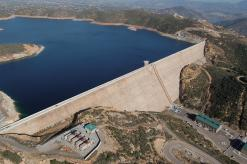
\includegraphics[width=\linewidth]{source-media/dam.jpeg}\end{column}
\end{columns}
\pause
\[S(x)=\frac{(a+b)x}{2}=\frac{(30+30+4x)x}{2}=2x^2+30x.\]
\alert{定义域为 $[10,50]$。}实际问题中，定义域受实际意义制约。
\end{frame}
% 原第5页
\begin{frame}[t]{解析法：计算与特点}
由 $S(x)=2x^2+30x$，得
\[S(15)=900\,\mathrm m^2,\quad S(20)=1400\,\mathrm m^2,\quad S(30)=2700\,\mathrm m^2.\]
\vspace{4mm}
\begin{block}{优点}
简洁明了，便于计算函数值和推导函数的性质。
\end{block}
\begin{block}{局限}
不够形象、直观；并不是所有函数都能用通常的解析式表示。
\end{block}
\end{frame}
% 原第6页
\begin{frame}[t]{新知探索：列表法}
商店里某商品每件价格为 $1.45$ 元，为方便查阅，可以列出下表。
\vspace{4mm}
\begin{center}\small\setlength{\tabcolsep}{3.2pt}
\begin{tabular}{c*{10}{r}}\toprule
数量/件&1&2&3&4&5&6&7&8&9&10\\\midrule
金额/元&1.45&2.90&4.35&5.80&7.25&8.70&10.15&11.60&13.05&14.50\\\bottomrule
\end{tabular}\end{center}
\vspace{3mm}
\begin{block}{列表法}
用表格列出自变量的值及其对应函数值来表示函数的方法。
\end{block}
这里，自变量是商品的件数，相应金额是商品件数的函数。
\end{frame}
% 原第7页
\begin{frame}[t]{列表法：水深与存水量}
某水库的存水量 $Q$（单位：$10^4\,\mathrm m^3$）与水库最深处水深 $H$（单位：$\mathrm m$）的关系如下表。
\vspace{5mm}
\begin{center}\renewcommand{\arraystretch}{1.5}
\begin{tabular}{c*{7}{r}}\toprule
$H/\mathrm m$&5&10&15&20&25&30&35\\\midrule
$Q/(10^4\,\mathrm m^3)$&20&40&90&160&275&437&650\\\bottomrule
\end{tabular}\end{center}
\vspace{3mm}
从表中可以看到，每个列出的水深 $H$ 都对应唯一的存水量 $Q$。
\alert{这张表给出了这些水深取值对应的函数值。}
\end{frame}
% 原第8页
\begin{frame}[t]{列表法：特点与应用}
\begin{columns}[T,onlytextwidth]
\begin{column}{.48\textwidth}
\begin{block}{优点}
具体易用，便于直接查表。\par
对于已列出的自变量值，可以直接查到对应函数值。
\end{block}
\end{column}
\begin{column}{.48\textwidth}
\begin{block}{局限}
当只列出部分数据时，信息不够全面。\par
通常不易直接看出整体变化规律。
\end{block}
\end{column}\end{columns}
\vspace{3mm}
\dinosay{储蓄利率表、汽车折旧保费表、税率表……你还能举出哪些例子？}
\end{frame}
% 原第9页
\begin{frame}[t]{新知探索：图象法}
\begin{columns}[c,onlytextwidth]
\begin{column}{.63\textwidth}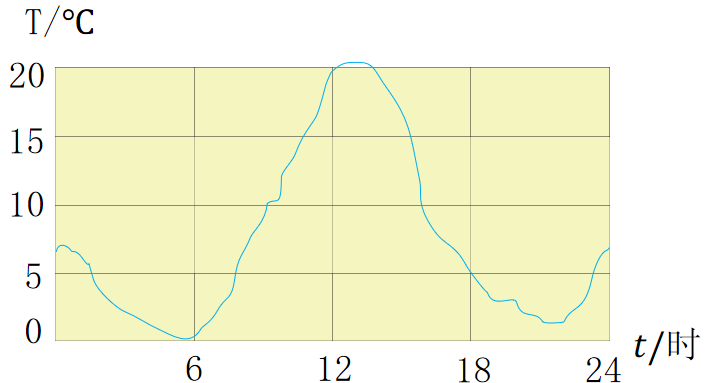
\includegraphics[width=\linewidth,height=48mm,keepaspectratio]{source-media/temperature.png}\end{column}
\begin{column}{.34\textwidth}
这是自动测温仪测得的某地某日 $0$ 时至 $24$ 时的温度曲线。
\par\alert{说一说}
\begin{itemize}
\item 下午 $2$—$3$ 时的气温大约是多少？
\item 何时气温最低？
\end{itemize}
\end{column}\end{columns}
\end{frame}
% 原第10页
\begin{frame}[t]{图象法：列表、描点、连线}
为了直观地了解函数的性质，常要作出函数的图象。
\begin{description}
\item[列表] 在定义域内选取有代表性的自变量值 $x$，计算对应的函数值 $f(x)$，列成表格。
\item[描点] 在平面直角坐标系中描出点 $(x,f(x))$。
\item[连线] 对于可连续连线的部分，按自变量从小到大的顺序，用适当的曲线连接。
\end{description}
\vspace{3mm}
\dinosay{描点前先看定义域。离散的点不能随意连成线。}
要作出更精确的图象，通常需要描出更多有代表性的点。
\end{frame}
% 原第11页
\begin{frame}[t]{例题解析：平方根函数的图象}
作出函数 $y=\sqrt{x}$，$x\in[0,16]$ 的图象。
\begin{center}\small\renewcommand{\arraystretch}{1.35}
\begin{tabular}{c*{8}{c}}\toprule
$x$&0&$\frac14$&1&$\frac94$&4&$\frac{25}4$&9&16\\\midrule
$y$&0&$\frac12$&1&$\frac32$&2&$\frac52$&3&4\\\bottomrule
\end{tabular}\end{center}
\pause
\begin{columns}[c,onlytextwidth]
\begin{column}{.56\textwidth}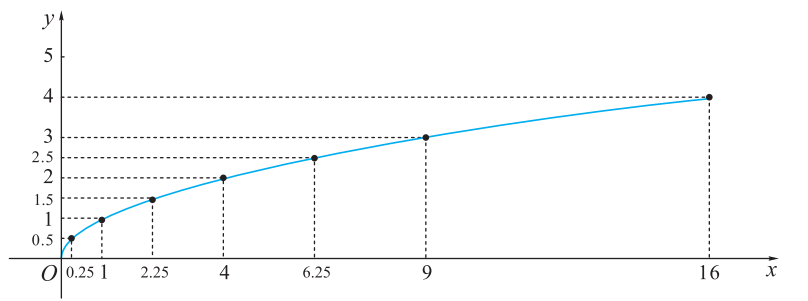
\includegraphics[width=\linewidth]{source-media/sqrt.png}\end{column}
\begin{column}{.41\textwidth}
\alert{优点：}形象、直观地表现函数的变化情况。\par
\alert{局限：}通常只能估读函数值，难以直接得到精确值。
\end{column}\end{columns}
\end{frame}
% 原第12页
\begin{frame}[t]{不同表示法与数形结合}
函数的三种表示方法各有长处和不足，研究具体问题时常把不同方法结合起来。
\begin{block}{数形结合}
用解析式计算与推理，用图象观察与验证。
\end{block}
\small
\textbf{其他表示方法}
\begin{itemize}
\item 标尺法：例如用带刻度的尺子测量油箱油深，再表示油量。
\item 算法或程序：用计算步骤表示某些函数。
\item 描述法：例如狄利克雷函数
\end{itemize}
\[D(x)=\begin{cases}1,&x\text{ 为有理数},\\0,&x\text{ 为无理数}.\end{cases}\]
\end{frame}
% 原第13页
\begin{frame}[t]{典例1：彩电销售的三种表示}
某商场新进了 $10$ 台彩电，每台售价 $3000$ 元。求售出台数 $x$（$x$ 为正整数）与收款数 $y$ 之间的函数关系，分别用列表法、图象法、解析法表示。
\pause
\vspace{5mm}
\alert{（1）列表法}
\begin{center}\small\setlength{\tabcolsep}{3.5pt}\renewcommand{\arraystretch}{1.5}
\begin{tabular}{c*{10}{r}}\toprule
$x$/台&1&2&3&4&5&6&7&8&9&10\\\midrule
$y$/元&3000&6000&9000&12000&15000&18000&21000&24000&27000&30000\\\bottomrule
\end{tabular}\end{center}
\end{frame}
% 原第14页
\begin{frame}[t]{典例1：图象与解析式}
\begin{columns}[c,onlytextwidth]
\begin{column}{.45\textwidth}
\alert{（2）图象法}\par
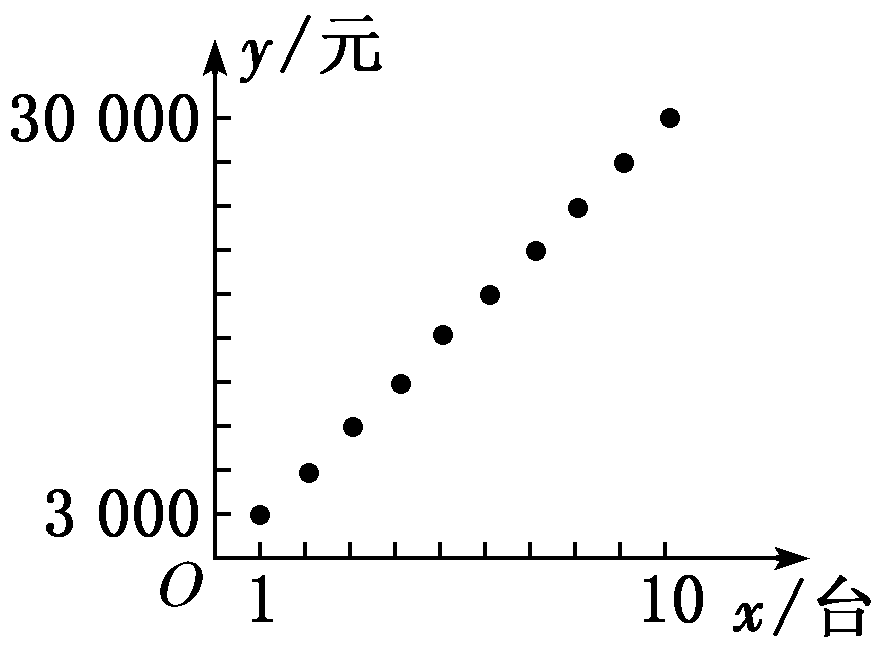
\includegraphics[height=43mm]{source-media/sales.png}
\end{column}
\begin{column}{.52\textwidth}
\alert{（3）解析法}
\[y=3000x,\quad x\in\{1,2,\ldots,10\}.\]
\dinosay{图象只有10个点，不能把这些点连成线。}
\end{column}\end{columns}
\end{frame}
% 原第15页，修正过强的适用前提
\begin{frame}[t]{方法提炼：三种表示法的选择}
解析法、列表法和图象法，从不同角度刻画自变量与函数值的对应关系。
\begin{itemize}
\item 有适当的解析式时，解析法便于精确计算与推理。
\item 需要观察整体变化时，图象法更直观。
\item 数据有限或需要查值时，列表法更方便。
\end{itemize}
\begin{block}{表示时的注意点}
（1）解析法必须交代定义域。\par
（2）完整的函数表应列出定义域内所有输入及对应输出；部分数据表只能提供部分信息。\par
（3）图象法必须明确图象是离散的点，还是可以连续连接的线。
\end{block}
\end{frame}
% 原第16页
\begin{frame}[t]{典例2：作图并求值域}
作出下列函数的图象，并求出其值域。
\vspace{3mm}
\begin{enumerate}
\setlength{\itemsep}{6mm}
\item $y=2x+1,\quad x\in[0,2]$；
\item $y=\dfrac2x,\quad x\in[2,+\infty)$；
\item $y=x^2+2x,\quad x\in[-2,2]$。
\end{enumerate}
\end{frame}
% 原第17页
\begin{frame}[t]{典例2：定义域决定图象范围}
\begin{columns}[T,onlytextwidth]
\begin{column}{.30\textwidth}
\centering $y=2x+1$\par $x\in[0,2]$\par
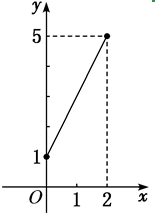
\includegraphics[height=30mm]{source-media/linear.png}\par
值域：\alert{$[1,5]$}
\end{column}
\begin{column}{.32\textwidth}
\centering $y=\dfrac2x$\par $x\in[2,+\infty)$\par
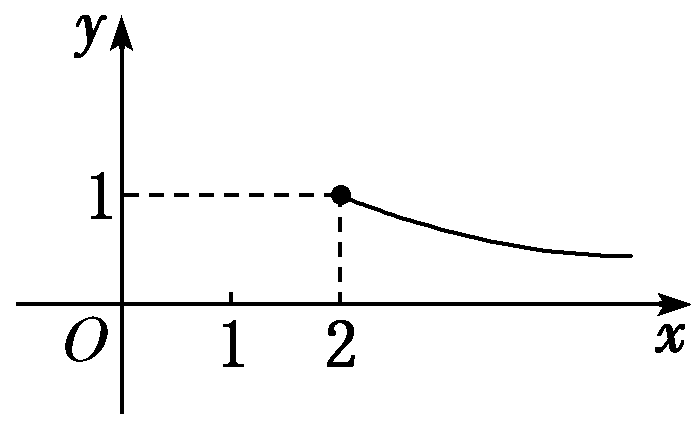
\includegraphics[width=\linewidth,height=30mm,keepaspectratio]{source-media/reciprocal.png}\par
值域：\alert{$(0,1]$}
\end{column}
\begin{column}{.30\textwidth}
\centering $y=(x+1)^2-1$\par $x\in[-2,2]$\par
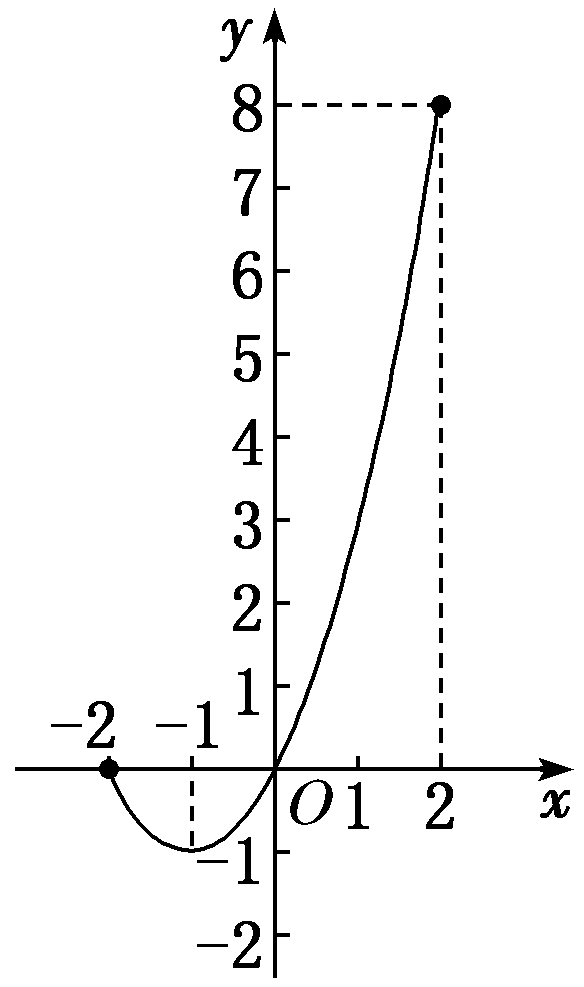
\includegraphics[height=30mm]{source-media/quadratic.png}\par
值域：\alert{$[-1,8]$}
\end{column}\end{columns}
\vspace{3mm}
\centering 注意端点是否取到，以及顶点是否位于定义域内。
\end{frame}
% 原第18页
\begin{frame}[t]{方法提炼：描点作图的关注点}
\begin{enumerate}
\setlength{\itemsep}{4mm}
\item 首先关注定义域，只在定义域内作图。
\item 实际图象用实线或实点表示；定义域外的辅助部分可用虚线表示。
\item 标出顶点、端点、与坐标轴的交点等关键点，分清实心点与空心圈。
\end{enumerate}
\vspace{3mm}
\dinosay{函数图象可以是曲线、直线、折线，也可以是离散的点。}
\end{frame}
% 原第19页
\begin{frame}[t]{典例3：求函数的解析式}
\small
（1）已知 $f(\sqrt{x}+1)=x+2\sqrt{x}$，求 $f(x)$。\par
（2）已知 $f(x)$ 是二次函数，且 $f(0)=1$，$f(x+1)-f(x)=2x$，求 $f(x)$。\par
（3）已知对任意实数 $x$，都有 $f(x)-2f(-x)=1+2x$，求 $f(x)$。
\pause
\begin{block}{（1）换元法}
令 $t=\sqrt{x}+1$，则 $x=(t-1)^2$，且 $t\ge1$。
\[f(t)=(t-1)^2+2(t-1)=t^2-1.\]
因此，$f(x)=x^2-1$，$x\ge1$。
\end{block}
只能由已知条件确定 $[1,+\infty)$ 上的函数值。
\end{frame}
% 原第20页
\begin{frame}[t]{典例3（1）：配凑法}
已知 $f(\sqrt{x}+1)=x+2\sqrt{x}$。
\vspace{3mm}
\begin{align*}
x+2\sqrt{x}&=(\sqrt{x})^2+2\sqrt{x}+1-1\\
&=(\sqrt{x}+1)^2-1.
\end{align*}
所以 $f(\sqrt{x}+1)=(\sqrt{x}+1)^2-1$。
\[\boxed{f(x)=x^2-1,\quad x\ge1.}\]
\dinosay{配凑出整体后，还要确定这个整体的取值范围。}
\end{frame}
% 原第21页
\begin{frame}[t]{典例3（2）：待定系数法}
设 $f(x)=ax^2+bx+c$，其中 $a\ne0$。由 $f(0)=1$，得 $c=1$。
又因为 $f(x+1)-f(x)=2x$，所以
\[a(x+1)^2+b(x+1)+1-(ax^2+bx+1)=2x.\]
整理得
\[2ax+(a+b)=2x.\]
比较对应项系数：
\[\begin{cases}2a=2,\\a+b=0,\end{cases}\qquad
\begin{cases}a=1,\\b=-1.\end{cases}\]
\[\boxed{f(x)=x^2-x+1.}\]
\end{frame}
% 原第22页
\begin{frame}[t]{典例3（3）：解方程组法}
已知对任意实数 $x$，有
\[f(x)-2f(-x)=1+2x.\]
以 $-x$ 代替 $x$，得 $f(-x)-2f(x)=1-2x$。
\pause
联立：
\[\begin{cases}f(x)-2f(-x)=1+2x,\\f(-x)-2f(x)=1-2x.\end{cases}\]
第一式加上第二式的 $2$ 倍，得 $-3f(x)=3-2x$。
\[\boxed{f(x)=\frac23x-1.}\]
\end{frame}
% 原第23页
\begin{frame}[t]{方法提炼：解析式的四种求法}
\small\renewcommand{\arraystretch}{1.8}
\begin{tabular}{p{23mm}p{111mm}}\toprule
方法&适用线索与注意点\\\midrule
配凑法&已知 $f(g(x))=F(x)$，把 $F(x)$ 改写成关于 $g(x)$ 的式子；注明 $g(x)$ 的取值范围。\\
待定系数法&已知函数类型，如一次函数或二次函数，先设一般形式，再用条件确定系数。\\
换元法&已知复合函数的解析式，令 $t=g(x)$；注意新变量的取值范围。\\
解方程组法&条件同时涉及 $f(x)$ 与 $f(-x)$ 或 $f(1/x)$，通过代换构造另一等式，联立消元。\\\bottomrule
\end{tabular}
\end{frame}
% 原第24页
\begin{frame}[t]{习题补充1：求解析式}
根据条件求下列函数的解析式。
\begin{enumerate}
\setlength{\itemsep}{6mm}
\item 已知 $f\left(x+\dfrac1x\right)=x^2+\dfrac1{x^2}$，求 $f(x)$。
\item 已知 $f(x)$ 是一次函数，且满足\par
$3f(x+1)-2f(x-1)=2x+17$，求 $f(x)$。
\item 已知 $2f(x)+f\left(\dfrac1x\right)=3x$，求 $f(x)$。
\end{enumerate}
\end{frame}
% 原第25页
\begin{frame}[t]{习题补充1：解析}
\small
（1）令 $t=x+\dfrac1x$，则 $t\in(-\infty,-2]\cup[2,+\infty)$。
\[x^2+\frac1{x^2}=\left(x+\frac1x\right)^2-2
\quad\Longrightarrow\quad f(t)=t^2-2.\]
故 $f(x)=x^2-2$，$x\le-2$ 或 $x\ge2$。
\medskip\par
（2）设 $f(x)=kx+b$（$k\ne0$），则 $kx+5k+b=2x+17$。
由 $k=2$、$5k+b=17$，得 $\boxed{f(x)=2x+7}$。
\medskip\par
（3）以 $1/x$ 代替 $x$，联立
\[\begin{cases}2f(x)+f(1/x)=3x,\\f(x)+2f(1/x)=3/x,\end{cases}
\quad\Longrightarrow\quad \boxed{f(x)=2x-\frac1x\ (x\ne0)}.\]
\end{frame}
% 原第26页
\begin{frame}[t]{习题补充2：求解析式}
\small
\begin{enumerate}
\setlength{\itemsep}{5mm}
\item 已知 $f\left(x+\dfrac1x\right)=x^3+\dfrac1{x^3}$，求 $f(x)$。
\item 若 $f\left(\dfrac1x\right)=\dfrac{x}{1-x}$（$x\ne0,1$），求 $f(x)$。
\item 已知 $f(x)$ 是一次函数，且满足\par
$3f(x+1)-2f(x-1)=2x+17$，求 $f(x)$。
\item 已知 $f(x)$ 的定义域为 $(0,+\infty)$，且\par
$f(x)=2f\left(\dfrac1x\right)\sqrt{x}-1$，求 $f(x)$。
\end{enumerate}
\end{frame}
% 原第27页
\begin{frame}[t]{习题补充2：（1）（2）解析}
\small
（1）利用恒等式
\[x^3+\frac1{x^3}=\left(x+\frac1x\right)^3-3\left(x+\frac1x\right).\]
当 $x>0$ 时，$x+1/x\ge2$；当 $x<0$ 时，$x+1/x\le-2$。
\[\boxed{f(x)=x^3-3x,\quad x\le-2\text{ 或 }x\ge2.}\]
\vspace{3mm}
（2）令 $t=1/x$，则 $t\ne0,1$，且
\[f(t)=\frac{1/t}{1-1/t}=\frac1{t-1}.\]
\[\boxed{f(x)=\frac1{x-1},\quad x\ne0,1.}\]
\end{frame}
% 原第28页
\begin{frame}[t]{习题补充2：（3）（4）解析}
\small
（3）设 $f(x)=ax+b$（$a\ne0$），则 $ax+5a+b=2x+17$。
由 $a=2$、$5a+b=17$，得 $\boxed{f(x)=2x+7}$。
\medskip\par
（4）由
\[f(x)=2\sqrt{x}\,f(1/x)-1\tag{1}\]
以 $1/x$ 代替 $x$，得
\[f(1/x)=\frac{2}{\sqrt{x}}f(x)-1.\tag{2}\]
将（2）代入（1）：$f(x)=4f(x)-2\sqrt{x}-1$。
\[\boxed{f(x)=\frac23\sqrt{x}+\frac13,\quad x>0.}\]
\end{frame}
% 原第29页
\begin{frame}[t]{课堂总结：函数的表示方法}
\renewcommand{\arraystretch}{1.7}
\begin{tabular}{p{26mm}p{105mm}}\toprule
解析法&用数学表达式表示自变量与函数值的对应关系。\\
列表法&用表格列出输入与对应输出。\\
图象法&用点集在坐标系中表示对应关系。\\
其他表示法&标尺法、算法或程序、描述法等。\\\bottomrule
\end{tabular}
\vspace{4mm}
\dinosay{表示函数，要交代清楚定义域和对应关系；研究函数，要善于数形结合。}
\end{frame}
% 原第30页，保留原稿作业页码
\begin{frame}[t]{课后作业}
\begin{enumerate}
\setlength{\itemsep}{7mm}
\item 课本第72页：练习1、2、3。
\item 课本第76页：习题3.1第2、3、7、8题。
\item 《三维设计》“函数的表示法”：\par 课时跟踪检测（十四）。
\end{enumerate}
\end{frame}
\campusclosing[本课结束]
